% do not change these two lines (this is a hard requirement
% there is one exception: you might replace oneside by twoside in case you deliver 
% the printed version in the accordant format
\documentclass[11pt,titlepage,oneside,openany]{book}
\usepackage{times}

\usepackage{enumitem}


\usepackage{graphicx}
\usepackage{latexsym}
\usepackage{amsmath}
\usepackage{amssymb}

\usepackage{ntheorem}

% \usepackage{paralist}
\usepackage{tabularx}

% this packaes are useful for nice algorithms
\usepackage{algorithm}
\usepackage{algorithmic}

% well, when your work is concerned with definitions, proposition and so on, we suggest this
% feel free to add Corrolary, Theorem or whatever you need
\newtheorem{definition}{Definition}
\newtheorem{proposition}{Proposition}


% its always useful to have some shortcuts (some are specific for algorithms
% if you do not like your formating you can change it here (instead of scanning through the whole text)
\renewcommand{\algorithmiccomment}[1]{\ensuremath{\rhd} \textit{#1}}
\def\MYCALL#1#2{{\small\textsc{#1}}(\textup{#2})}
\def\MYSET#1{\scshape{#1}}
\def\MYAND{\textbf{ and }}
\def\MYOR{\textbf{ or }}
\def\MYNOT{\textbf{ not }}
\def\MYTHROW{\textbf{ throw }}
\def\MYBREAK{\textbf{break }}
\def\MYEXCEPT#1{\scshape{#1}}
\def\MYTO{\textbf{ to }}
\def\MYNIL{\textsc{Nil}}
\def\MYUNKNOWN{ unknown }
% simple stuff (not all of this is used in this examples thesis
\def\INT{{\mathcal I}} % interpretation
\def\ONT{{\mathcal O}} % ontology
\def\SEM{{\mathcal S}} % alignment semantic
\def\ALI{{\mathcal A}} % alignment
\def\USE{{\mathcal U}} % set of unsatisfiable entities
\def\CON{{\mathcal C}} % conflict set
\def\DIA{\Delta} % diagnosis
% mups and mips
\def\MUP{{\mathcal M}} % ontology
\def\MIP{{\mathcal M}} % ontology
% distributed and local entities
\newcommand{\cc}[2]{\mathit{#1}\hspace{-1pt} \# \hspace{-1pt} \mathit{#2}}
\newcommand{\cx}[1]{\mathit{#1}}
% complex stuff
\def\MER#1#2#3#4{#1 \cup_{#3}^{#2} #4} % merged ontology
\def\MUPALL#1#2#3#4#5{\textit{MUPS}_{#1}\left(#2, #3, #4, #5\right)} % the set of all mups for some concept
\def\MIPALL#1#2{\textit{MIPS}_{#1}\left(#2\right)} % the set of all mips





\begin{document}

\pagenumbering{roman}
% lets go for the title page, something like this should be okay
\begin{titlepage}
	\vspace*{2cm}
  \begin{center}
   {\Large Project Report\\}
   \vspace{1cm} 
   {Predicting the Perfect Beer\\}
   \vspace{2cm}
   {    Michael Dell\\
    Marc Mengler\\
   }
   \vspace{2.5cm}
   {Web Mining Class} \\
   {Prof. Dr. Christian Bizer}\\
  % \vspace{1cm}
   {FSS 2014}
  \end{center}
\end{titlepage} 

% no lets make some add some table of contents
\tableofcontents
\newpage

%\listofalgorithms

%\listoffigures

%\listoftables

% evntuelly you might add something like this
% \listtheorems{definition}
% \listtheorems{proposition}

\newpage


% okay, start new numbering ... here is where it really starts
\pagenumbering{arabic}


% Project Summaries
% 
% 10-12 pages (sharp!) without title or toc pages 
% 
% due 
% 19.5.2014, 23:59
% 
% send by email to Chris, Cäcilia, Oliver, and Robert
% 
% describe your solution including the steps to get there:
% 1.
% Application domain and goals
% 2.
% Structure and size of the data set
% 3.
% Preprocessing
% 4.
% Actual Web Mining
% 5.
% Evaluation
% 6.
% Results
% 
% Requirements
% 
% You must use the DWS master thesis layout.
% 
% Please cite sources properly. Preferred citation style [Author, year].
% 
% Also submit your Rapid Miner pro
% cesses and (a subset) of your data.

\chapter{Introduction}
\label{cha:intro}


Plaintext reviews in combination with a single numeric overall score are quite commonly found in online platforms. They are then analyzed to serve as the basis for recommender systems, product summarisations and sentiment analyses. To maximise the value extracted from these reviews, one has to understand why users evaluate products the way they did. Was it due to the taste or the look of a beer that the user rated it as low-performing? Despite the taste or look, are there particular aspects that the user liked about the beer? And which words do users frequently use to indicate such preferences?

To overcome these challenges, prior research has shown that rating systems, which use explicit rating dimensions, are more accurate.%find sources
Explicit referring to rating each aspect of a product seperately. This goes along with our intuition. We presume that when users evaluate beer, their perception is driven by multiple senses, including a visual, olfactoric, gustatoric and tactile evaluation of the beer. To account for this, we use multi-aspect reviews which include the following four sensory aspects: the smell, taste, feel (palate) and look of a beer, in combination with the overall evaluation of it. 

However, instead of assigning complete reviews, we build a model which attempts to assign each sentence to one of the four explicit aspects. 





%include statistics about beer consumption
Statistics show: The amount of beer consumed is growing on a yearly basis. So is the amount of beer-connaisseurs who value the plentifulness and settle differences of each aspect of beer. 






\section{The Challenge}

%Michi:Etwas mehr bezug zur existing literature, zb:
%Usually authors try to gather general sentiment lexicons for their languages (Mihalcea et al., 2007; Banea et al., 2008; Clematide & Klenner, 2010; Steinberger et al., 2011).

The domain of beer is highly specialized and can not be analyzed using existing generic polarity lexicons. It requires polarity sentiment lexicon induction. This research aims to fill the gap for this specific domain, also answering the interesting domain question: What makes a good beer?
%Jap, ein kleiner literature review folgt spätestens Sonntag! 

\section{Dataset}

We base our research on multi-aspect user reviews from RateBeer.com. It is a free, community-supported online platform with fee-based premium features. It describes itself as "...widely recognized as the most accurate and most-visited source for beer information."\footnote{http://www.ratebeer.com/About.asp, retrieved May, 16th, 2014} Users register on this platform to rate and describe different aspects of all kinds of beer. 

An exemplaric entry: \\
\begin{quote}
appearance: 4/5
aroma: 10/10
palate: 5/5
taste: 8/10
overall: 20/20 \\
\emph{Wow! this one was amazing.  Aroma is chocolate, coffee, vanilla.  Appearance is jet black with nice tan head that dissipates to thin ring.  Lots of lace.  Taste is coffee, chocolate, vanilla, slight hops, heavy malt, oatmeal.  Palate is silky smooth, some lactose in there to smooth around the edges and sweeten a bit.  Overall, very impressed! I walked out of the brewery and saw they won a silver metal at the GABF.  Should have won gold!}
\end{quote}


All reviews undergo a moderation process where fake ratings as well as those of brewers or brewer-affiliates who rate their own product are deleted and their IP addresses tracked, among other measures to ensure the validity of RateBeer ratings.\footnote{http://www.ratebeer.com/ratingsqa.asp, retrieved May, 16th, 2014}. 

The 1.74~GB dataset at hand\footnote{Acknowledgement: The data set, part of the Stanford Network Analysis Project from http://snap.stanford.edu/data/web-RateBeer.html, is kindly provided with permission from RateBeer LLC and Stanford Assistant Professor Jure Leskovec.} consists of roughly 3 million reviews whereby each review depicts user ratings for four aspects of the beer, an overall rating score as well as a plaintext review with a median of 54 words. More statistics about the data set are illustrated in table~1.1. 


\begin{table}[h]
\label{tab:statistics}
\begin{center}

\begin{tabular}{|l|l|}
\hline
Number of reviews                  & 2,924,127           \\ \hline
Number of users                    & 40,213              \\ \hline
Number of beers                    & 110,419             \\ \hline
Median no. of words per review     & 54                  \\ \hline
Timespan                           & Apr 2000 - Nov 2011 \\ \hline
Aspect: Overall                    & scale 1-20, avg. 13.20 +/- 3.35 \\ \hline
Aspect: Appearance                 & scale 1-5,  avg. 3.43 +/- 0.81 \\ \hline
Aspect: Aroma                      & scale 1-10, avg. 6.35 +/- 1.64 \\ \hline
Aspect: Palate                     & scale 1-5,  avg. 3.26 +/- 0.83 \\ \hline
Aspect: Taste                      & scale 1-10, avg. 6.45 +/- 1.62 \\ \hline

\end{tabular}
\caption{Descriptive statistics for dataset}
\end{center}

\end{table}









\chapter{Our Approach}

%TODO:Adapt to actual work (Michi)
The first step with regard to the goal of the overall rating prediction of is to learn a model which is capable of predicting the overall rating with an acceptable accuracy. Furthermore we generate a domain specific polarity lexicon, since the language used in the reviews differs significantly from every day language. Subsequently, we adapt the lexicon deduction and the prediction model to work on aspect level in order to achieve more fine-grained results. Lastly, we investigate possibilities for summarization, meaning identifying a subset of words and sentences which best explain several reviewers' multiple-aspect rating and visualize them in an appropriate way.




\section{Preprocessing}

The dataset requires pre-processing. Since it is an international data set and we learn an english sentiment lexicon, we filter a total of 38019 non-english reviews, accounting for 1.3 per cent of total reviews being excluded. This leads to a total of 2,886,144 reviews which are assigned to three equal-sized stratified samples, two of which are used for training and one of which is used for testing purposes. Since the review forms used by RateBeer.com require users to rate each of the 5 aspects and to describe the beer, theoretically, the dataset does not contain missing values. Practically, we ensure this quality-level by filtering for missing values implicitly.

To ensure quality of our sentiment polarity, we exclude reviews with an overall rating of 12, 13 and 14. 

Furthermore, the text mining analysis requires additional pre-processing, all settings of which are intentionally implemented on a flexible basis, to be able to determine best-performing experiments. These include stop-word removal, tokenisation and lemmatisation. Since stopwords might contain valuable sentiment information, for stopword-removal, only a basic dictionary of 319 stopwords are used. Furthermore, POS tagging is used for all nouns, adjectives and adverbs.



\section{Lexicon Induction}

%TODO:Describe approach (Michi)

Our lexicon induction process aims to create four distinct lexicons, one for each of the four aspects \emph{appearance, aroma, taste,} and \emph{palate}.
The process on a high level is illustrated in the steps below and will be explained in detail afterwards.

\begin{enumerate}[noitemsep]
  \item Filter significantly low and high rated reviews with regards to each aspect
  \item From those filtered lists extract all sentences talking about the specific aspect
  \item Create a document for each of the lists by concatenating these sentences
  \item Transform each document in a word vector using tf-idf scores
  \item For each word in this vector:
    \begin{enumerate}[noitemsep]
    \item Decide for which aspect to include
    \item Determine final sentiment score
  \end{enumerate}
\end{enumerate}

\textbf{Step (1) Filtering reviews based on their aspect rating:} In order to take into account the different rating scales for different aspects we use a relative threshold for each of the two classes. If a review is included is determined by the formula $R_A/MAX(R_A) \ge T_{minTop}$ for the top class and $R_A/MAX(R_A) \le T_{maxLow}$ for the low class, whereby $R_A$ denotes the aspect rating and the respective $T \in [0,1]$ is a configurable threshold. This gives us a total of 8 lists, two for each aspect.\\

\textbf{Step (2) Aspect based sentence extraction:} For the sentence splitting task we use again Stanford CoreNLP tools. The sentence aspect mapping is done by a simple rule-based heuristic based on the occurrence of manually entered keywords, which are given in the table \ref{tab:keywords}. We argue that our corpus is large enough to allow us to ignore any ambiguous sentences.

\begin{table}[h]
\label{tab:keywords}
\begin{center}
\begin{tabular}{|l|l|}

\hline
\textbf{Aspect} & \textbf{Keyword(s)}                   \\ \hline
Appearance      & appearance, color, colour, look, head \\ \hline
Aroma           & aroma                                 \\ \hline
Palate          & palate                                \\ \hline
Taste           & taste, flavor, flavour                \\ \hline

\end{tabular}
\caption{Keywords for aspect determination}
\end{center}
\end{table}

\textbf{Step (3+4): Document and word vector creation:} The document creation is done in a straight forward manner by concatenating all extracted sentences from the previous step. For the word vector creation we use the WEKA machine learning library, treating each document as a single instance and applying their StringToWordVector class using tf-idf transformation. An example excerpt is shown in figure~\ref{fig:wordvector}. For a list of the used configuration parameters see section TODO.

\begin{figure}[h]
  \label{fig:wordvector}
  \centering
    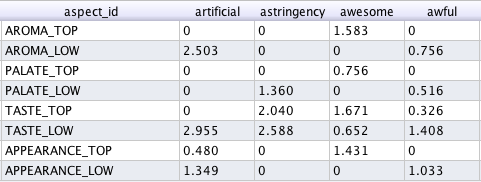
\includegraphics[width=0.6\textwidth]{wordvector}
    \caption{Excerpt from a resulting word vector}
\end{figure}


\textbf{Step (5): Actual lexica creation:} As indicated above this is done by looping over each word in the vector and first determine the lexicon i.e. the aspect it represents best. Second, calculating the final sentiment score it will get assigned with regards to the aspect. The aspect $a_w$ for each word is assigned by the maximum of the sums over the aspect's score: 
$\underset{a \in A}{\max} (\mbox{$TOP_a$}(w) + \mbox{$LOW_a$}(w))$ \\
Afterwards the final sentiment score of the word $S_w$ is calculated by the formula: $S_w = TOP_{a_w}(w) - LOW_{a_w}(w)$ These scores are then compiled in simple text based word lists, which can be applied in different scenarios. As part of this work we use them exemplarily to predict the overall rating of an unseen review.



%find papers about the but-multiplier
\section{Rating Prediction}

In the following we will describe our approach to predict the overall rating of an unseen review by using our created sentiment lexica to calculate a sentiment score of the review's text. This, on the one hand can be seen as an evaluation of the quality of our compiled sentiment lexica, but on the other hand is a challenging task in general. Therefore we describe our approach in detail. The results and the overall evaluation can then be found in chapter TODO.\\
In the scope of this project we handle the rating prediction task as a two-class classification problem, i.e. we introduce a binary label \emph{IS\_OVERALL\_TOP} for a review $r$ according to the following formula:
\[ Label(r) = \left\{ 
  \begin{array}{l l}
    true & \quad \text{if $n$}\\
    false & \quad \text{if $n$}
  \end{array} \right.\]

For each unseen review we take only the review's freetext into account. NLP-wise we apply the same pre-processing steps to this text as we applied for the lexicon creation step, i.e. especially 

\section{Experiments}
TODO:Describe experiment setup and configuration parameters ...\\


%Michi:Würde hier nur die wirklich für die wordlist induction relevanten parameter auflisten
As with pre-processing, we intentionally implemented all parameters on a flexible basis, to be able to determine best settings in multiple experiments. A complete list of parameters are depicted in table 2.1.

%Michi:Eventuell generell nur für experimmente relevante parameter auflisten
\begin{table}[h]
\label{tab:Parameters for Testing}
\begin{center}

\begin{tabular}{|l|l|}
\hline
Number of reviews loaded           & max. 2,886,144           \\ \hline
Text Analysis          &      \\ \hline
POS tags                   & which POS to include               \\ \hline
useLemma                  & true or false          \\ \hline
includePOS                  & true or false          \\ \hline
Annotators     & tokenize, ssplit, pos, lemma                  \\ \hline
Wordlist creation parameters     &                \\ \hline
idfTransform                           & true or false \\ \hline
outputWordCounts                            & true or false\\ \hline
lowerCaseTokens                   & true or false \\ \hline
useStoplist                & true or false \\ \hline
stopwordsFile                     & path to .txt \\ \hline
wordsToKeep                     & max. amount of words for all 4 dictionaries \\ \hline
minTermFreq                    & specifies min threshold a word has to occur \\ \hline
Thresholds                   &  \\ \hline
minTopRatingScore                  & specifies min threshold for top class in per cent \\ \hline
maxLowRatingScore                  & specifies max threshold for low class in per cent \\ \hline
Evaluation Parameters                   &  \\ \hline
minTopClassScore                  & 0.7 to match average rating of 13.37 for aspect overall \\ \hline
minSentimentTopScore                  & 0.0 to demonstrate equal distribution of dictionaries\\ \hline
butMultiplier                 & specifies an amplifier for but-occurrences \\ \hline
\end{tabular}
\caption{Parameters for Experiments}
\end{center}

\end{table}

Settings for parameters of each experiment are determined manually, but logged automatically to record performance deviations for re-adjustment of parameters. For each experiment we measure accuracy, precision, recall, f1-score, average sentiment and the percentage of the special case of but-occurrences using a three-fold cross validation. The occurrence of but in a sentence has the potential to change the meaning and sentiment significantly. To account for it, we decide to give additional weighting to the words preceding but, optimal settings are determined on experimentation-basis.






\chapter{Evaluation and Discussion}

In this section, the results of a total of XXXX experiments are discussed and compared with related studies.
 

\section{Evaluation}


\section{Results}

\section{Discussion}

%The evaluation will also include a comparison with the results of related studies, especially from Stanford researchers McAuley et al. (2012)\footnote{McAuley, J., Leskovec, J., & Jurafsky, D. (2012, December). Learning attitudes and attributes from multi-aspect reviews. In Data Mining (ICDM), 2012 IEEE 12th International Conference on (pp. 1020-1025). IEEE.}, who performed similar research using the rateBeer.com data set as one data sources.  We expect our generated polarity database, the summarization and prediction to perform accurately and significantly better than a generic polarity database in this real-world setting. 

\chapter{Conclusion and Future Work}
//TODO:Conclusion\\
Due to the limited scope of this project we were not able to empirically evaluate all variants of our approach. Nevertheless, we assume that slightly different variations of our approach could enhance the performance of our model and thus, could lay out the basis for future work in this field.

\section{Regarding the Lexicon Induction}

\section{Regarding the Classification Task}


\bibliographystyle{plain}
\bibliography{thesis-ref}



\end{document}
